\documentclass[tikz,border=3pt]{standalone}
\usepackage{tikz}
\usetikzlibrary{arrows.meta,positioning,calc,shapes.misc,fit,backgrounds}

% 简化集合书写
\newcommand{\set}[1]{\{#1\}}

% 统一样式
\tikzset{
  concept/.style={draw=black!55, fill=black!20, rounded corners=2pt,
                  inner xsep=5pt, inner ysep=3pt, font=\footnotesize},
  flow/.style={-Stealth, line width=0.6pt},
  hint/.style={-Stealth, dashed, gray, line width=0.5pt},
}

\begin{document}
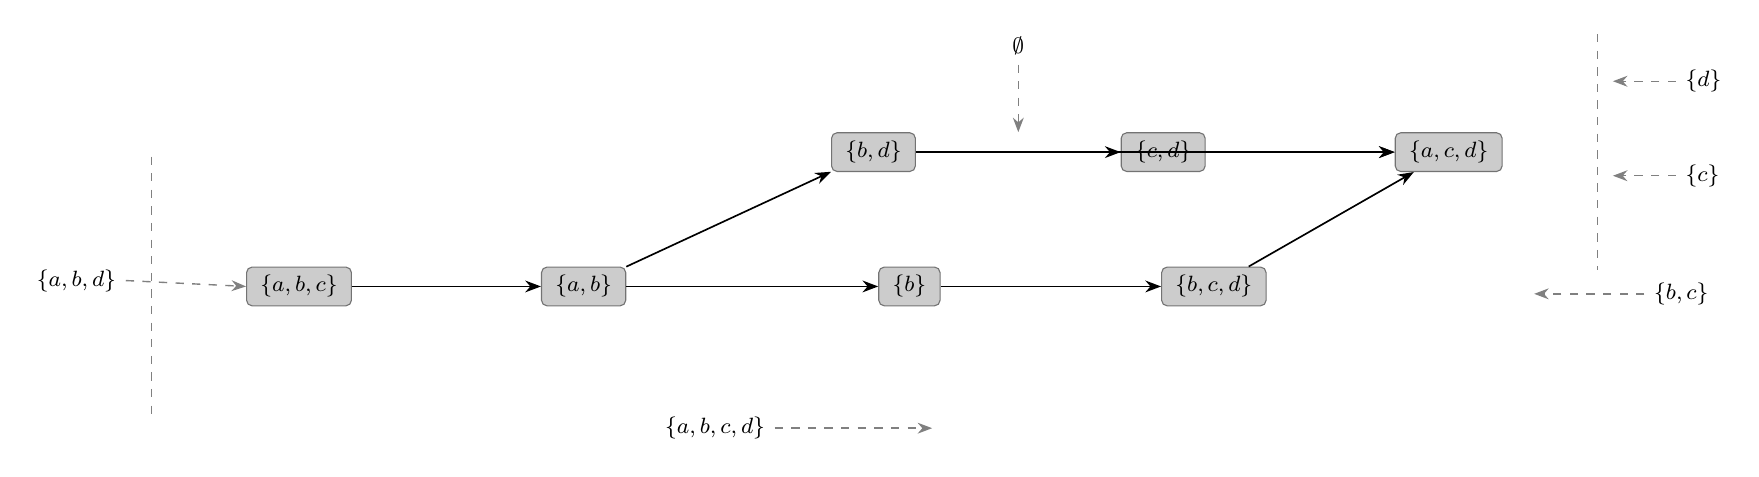
\begin{tikzpicture}[x=2.0cm, y=1.5cm]

% --- 节点(手动坐标,接近原图排布) ---
\node[concept]                          (abc) at (0, 0)   {$\set{a,b,c}$};
\node[concept, right=1.2 of abc]        (ab)               {$\set{a,b}$};

\node[concept, above right=0.8 and 1.3 of ab] (bd)         {$\set{b,d}$};
\node[concept, right=1.3 of bd]         (cd)               {$\set{c,d}$};

\node[concept, right=1.6 of ab]         (b)                {$\set{b}$};
\node[concept, right=1.4 of b]          (bcd)              {$\set{b,c,d}$};

\node[concept, right=1.2 of cd]         (acd)              {$\set{a,c,d}$};

% --- 实线关系(方向:左 -> 右) ---
\draw[flow] (abc) -- (ab);
\draw[flow] (ab)  -- (bd);
\draw[flow] (ab)  -- (b);
\draw[flow] (bd)  -- (cd);
\draw[flow] (bd)  -- (acd);
\draw[flow] (cd)  -- (acd);
\draw[flow] (b)   -- (bcd);
\draw[flow] (bcd) -- (acd);

% --- 外侧标签与虚线引导(位置可微调) ---
% 左侧标签 {a,b,d}
\node[anchor=east, font=\footnotesize] (Lleft) at (-1.10,0.05) {$\set{a,b,d}$};
\draw[hint] (Lleft.east) -- (abc.west);

% 上侧空集 ∅
\node[font=\footnotesize] (TopLab) at ($(bd)!0.5!(cd)+(0,0.90)$) {$\emptyset$};
\draw[hint] (TopLab.south) -- ($(bd.north)!0.5!(cd.north)$);

% 右侧参考虚线与两个标签 {d}、{c}
% 竖直虚线参考(只作视觉引导,可删)
\draw[dashed, gray] ($(acd.east)+(0.60, 1.0)$) -- ($(acd.east)+(0.60, -1.0)$);
\node[anchor=west, font=\footnotesize] (R1) at ($(acd.east)+(1.10, 0.60)$) {$\set{d}$};
\node[anchor=west, font=\footnotesize] (R2) at ($(acd.east)+(1.10,-0.20)$) {$\set{c}$};
\draw[hint] (R1.west) -- ++(-0.40,0); % 可改为指向 (acd.north east) 等
\draw[hint] (R2.west) -- ++(-0.40,0);

% 下侧两个标签 {a,b,c,d} 与 {b,c}
\node[font=\footnotesize] (BottomAll) at ($(ab)!0.5!(b)+(-0.20,-1.20)$) {$\set{a,b,c,d}$};
\draw[hint] (BottomAll.east) -- ++(1.00,0);

\node[anchor=west, font=\footnotesize] (BottomBC) at ($(acd.east)+(0.90,-1.20)$) {$\set{b,c}$};
\draw[hint] (BottomBC.west) -- ++(-0.70,0);

% 左侧竖直虚线(呼应右侧,纯装饰)
\draw[dashed, gray] ($(abc.west)+(-0.60, 1.10)$) -- ($(abc.west)+(-0.60, -1.10)$);

\end{tikzpicture}
\end{document}